\section{Esercizio 26}
\textit{\textbf{Descrizione:}  Scrivere una function che implementi efficientemente un metodo iterativo, per risolvere un sistema lineare, definito da un generico splitting della matrice dei coefficienti.}\newline
\emph{Soluzione: }\\~\\
\textbf{Splitting generico:}
\\~\\
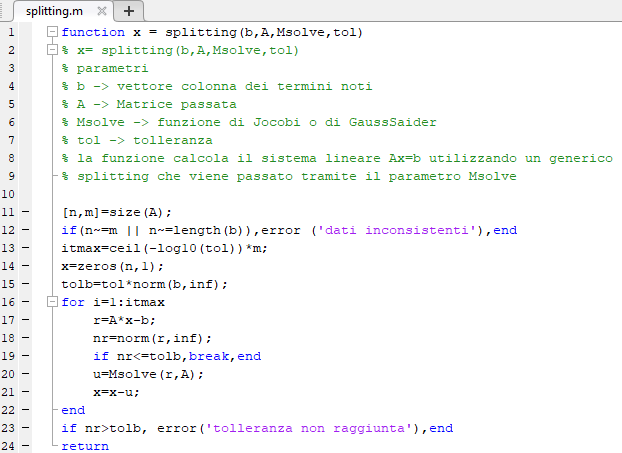
\includegraphics[width=1.3\linewidth]{img/splitting} \newpage